\documentclass[11pt,draftcls,onecolumn,peerreview]{IEEEtran}
\bibliographystyle{plain}
\usepackage{graphicx}
\usepackage{amssymb}
\usepackage{amsmath}
\usepackage[bbgreekl]{mathbbol}
\DeclareMathOperator*{\argmax}{argmax}
\DeclareMathOperator*{\argmin}{argmin}
\usepackage[affil-it]{authblk}
\usepackage{paralist}
\usepackage{url}
\usepackage{tabularx}
\usepackage{color}
\usepackage{tikz}
\usepackage{tipa}\newcommand{\ipa}[1]{\textipa{#1}}
\usepackage{stackrel}
\usetikzlibrary{positioning,shadows,arrows,shapes,calc}
\setlength{\textwidth}{6.5in}
\setlength{\textheight}{9in}
\setlength{\oddsidemargin}{0in}
\setlength{\topmargin}{0in}
\begin{document}

\begin{center}
  \tikzstyle{pre}=[<-,shorten <=1pt,>=stealth',semithick,draw=black]
  \tikzstyle{post}=[->,shorten >=1pt,>=stealth',semithick,draw=black]
  \begin{tikzpicture}[
      state/.style={circle,thick, draw=black, text=black, text width=0.25cm},
      compose/.style={circle,thick, draw=black, text=black, text width=0.1cm},
    ]
    \node[state] (g0) at (-1.5,1) {};
    \node[state] (g1) at (1.5,1) {};
    \node[state] (g2) at (0,-1) {};
    \draw[post] (g0) -- (-1.75,1.5) -- (-1.5,1.75) -- (-1.25,1.5) -- (g0);
    \draw[post] (g1) -- (1.25,1.5) -- (1.5,1.75) -- (1.75,1.5) -- (g1);
    \draw[post] (g2) -- (0.25,-1.5) -- (0,-1.75) -- (-0.25,-1.5) -- (g2);
    \draw[post] (g0) -- (g1);
    \draw[pre] (g0) -- (g2);
    \draw[pre] (g2) -- (g1);
    \draw[pre] (g0) -- (-1,1.5) -- (1,1.5) -- (g1);
    \draw[post] (g0) -- (-1.65,0.2) -- (-0.75,-1) -- (g2);
    \draw[post] (g2) -- (0.75,-1) -- (1.65,0.2) -- (g1);
    \node at (0,1.75) {a:a$/p(a|b)$};
    \node at (0,0.75) {b:b$/p(b|a)$};
    \node at (-2,-0.5) {\#0:$\epsilon$$/\beta(a)$};
    \node at (-0.45,0.1) {a:a};
    \node at (2,-0.5) {b:b$/p(b)$};
    \node at (0.4,0.15) {\#0:$\epsilon$};
    \node at (-1.5,2) {\#2:\#2};
    \node at (1.5,2) {\#2:\#2};
    \node at (0,-2) {\#2:\#2};
    \node[compose] (c) at (4,0) {};
    \node[state] (pt0) at (6,0) {};
    \node[state] (pt1) at (8,0) {};
    \node[state] (pt2) at (10,0) {$\circ$};
    %\node[compose] (pt2inner) at (10,0) {};
    \draw[post] (pt0) -- (6.5,0.5) -- (7.5,0.5) -- (pt1);
    \draw[post] (pt0) -- (6.5,-0.5) -- (7.5,-0.5) -- (pt1);
    \draw[post] (pt1) -- (8.5,0.5) -- (9.5,0.5) -- (pt2);
    \draw[post] (pt1) -- (8.5,-0.5) -- (9.5,-0.5) -- (pt2);
    \node at (7,0.75) {a:a$/0.8$};
    \node at (7,-0.75) {\#2:$\emptyset$$/0.2$};
    \node at (9,0.75) {b:b$/0.8$};
    \node at (9,-0.75) {a:a$/0.2$};
  \end{tikzpicture}
\end{center}
\centerline{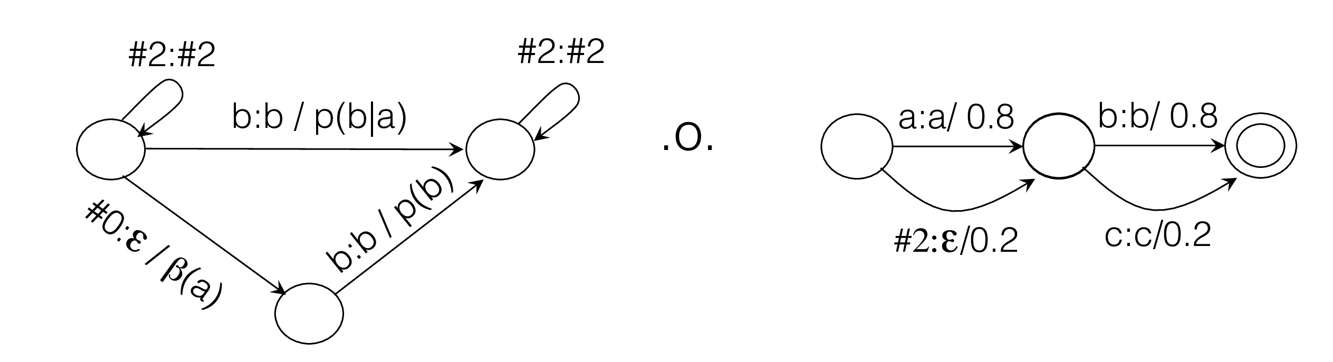
\includegraphics[width=5in]{../figs/liu1.png}}

\end{document}
